%Phần thiết đặt trang
\documentclass[12pt,a4paper]{article}
\usepackage[LGRgreek]{mathastext}
\usepackage[utf8]{vietnam}
\usepackage{amsfonts}
\usepackage{amsmath}
\usepackage{amssymb}
\usepackage{graphicx}
\usepackage[left=2cm,right=2cm,top=2cm,bottom=2cm]{geometry}
\setlength{\parindent}{0pt}
\usepackage{parskip}
\setlength{\parskip}{0.5em}


%Phần thiết kế khung code nhập liệu
\usepackage{listings}
\usepackage{color}

\definecolor{dkgreen}{rgb}{0,0.6,0}
\definecolor{gray}{rgb}{0.5,0.5,0.5}
\definecolor{mauve}{rgb}{0.58,0,0.82}

\lstset{frame=tb,
  language=C++,
  aboveskip=3mm,
  belowskip=3mm,
  showstringspaces=false,
  columns=flexible,
  basicstyle={\small\ttfamily},
  numbers=left,
  numberstyle=\small\color{gray},
  keywordstyle=\color{blue},
  commentstyle=\color{dkgreen},
  stringstyle=\color{mauve},
  breaklines=true,
  breakatwhitespace=true,
  tabsize=3
}

%Phần chọn font chèn câu lệnh giữa đoạn
\newenvironment{code}{\ttfamily}{\par}
\DeclareTextFontCommand{\chuyencode}{\code}

%Thêm chấm vào tiêu đề các phần
\usepackage{titlesec}
\titlelabel{\thetitle.\quad}

%Thêm định dạng cho các nút và menu lệnh.
\usepackage{menukeys}

%Nội dung chính
\begin{document}
%Chỉnh loại tiêu đề chương thành I, II
\renewcommand\thesection{\Roman{section}}
\renewcommand\thesubsection{\arabic{subsection}}
\renewcommand\thesubsubsection{\alph{subsubsection}}

%Mục lục
\tableofcontents

%Chương 1:
\section{Cơ bản về MATLAB}
\subsection{Không gian làm việc}
\subsubsection{Giao diện chính}
Có 3 cách khởi động chương trình Matlab từ máy tính chạy Windows:\\
- Khởi động từ biểu tượng ngoài màn hình.\\
- Mở trực tiếp tập tin có đuôi mở rộng là .m, ví dụ: Bai1.m hoặc Hamso.m\\
- Vào biểu tượng Start $>$ All Program $>$ MATLAB $>$ Matlab 2014b.\\
\begin{center}
    \begin{figure}[htp]
    \begin{center}
     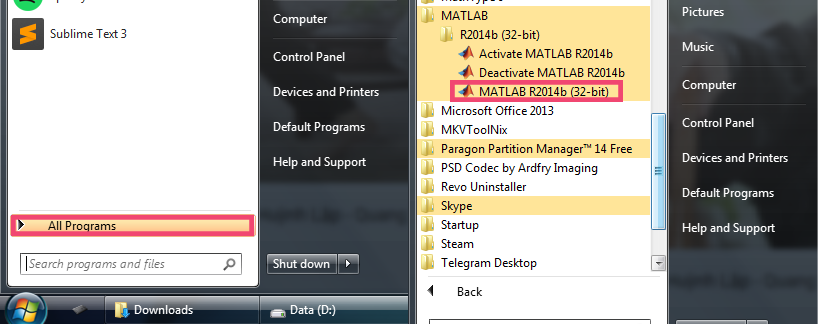
\includegraphics[scale=.7]{hinhtieuluan/pic1.png}
    \end{center}
    \caption{Thao tác mở chương trình từ Start Menu.}
    \label{refhinh1}
    \end{figure}
\end{center}
Giao diện chính của chương trình sau khi khởi động sẽ tương tự như hình bên dưới. Có 3 khu vực làm việc chính. Khung lớn nhất được bao viền màu xanh dương là Command Window. Khung Current Folder nằm ở phần trên, bên trái của Command Window. Phía dưới khung Current Folder là Khung Workspace.\\

\begin{center}
	\begin{figure}[htp]
	\begin{center}
		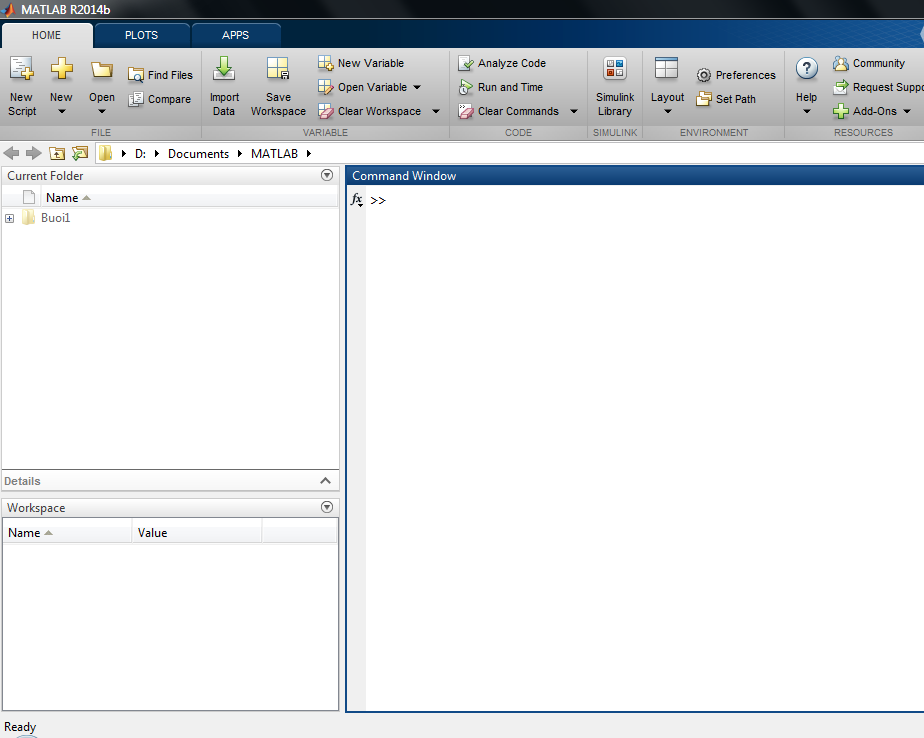
\includegraphics[scale=.6]{hinhtieuluan/pic2}
	\end{center}
		\caption{Giao diện chính của chương trình}
		\label{refhinh2}
	\end{figure}
\end{center}
Trong đó:\\
\begin{itemize}
	\item \textbf{Command Window:} Khu vực người dùng nhập các câu lệnh điều khiển và tính toán. Mỗi câu lệnh sẽ được thực hiện khi người dùng nhấn Enter.
	\item \textbf{Current Folder:} Khu vực truy cập các tập tin m-file, m-hàm... được lưu trữ trên ổ đĩa máy tính.
	\item \textbf{Workspace:} Liệt kê các biến và dữ liệu đang được xử lý tạm thời. Ngoài ra người dùng có thể thao tác thêm bớt chỉnh sửa các giá trị của biến và tham số trực tiếp trên Workspace mà không cần dùng đến câu lệnh.
\end{itemize}
Ngoài ba khu vực chính trên, kể từ phiên bản MATLAB 2012a, thanh công cụ phía trên cùng truyền thống đã được thay thế bằng các thẻ lệnh Ribbon với biểu tượng cụ thể và rõ ràng hơn.\\
\begin{center}
	\begin{figure}[htp]
		\begin{center}
		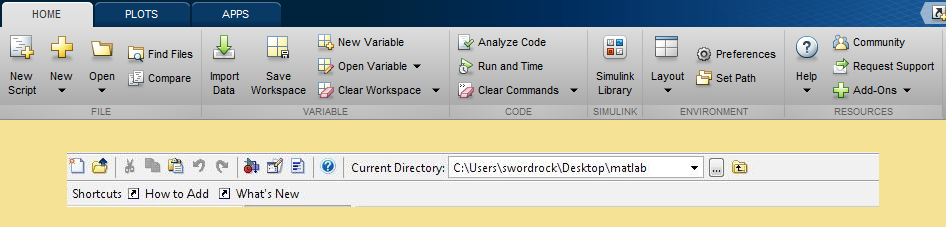
\includegraphics[scale=.5]{hinhtieuluan/pic3}
		\end{center}
		\caption{Thẻ Home (hình trên) ở giao diện mới và thanh công cụ truyền thống (hình dưới)}
		\label{refhinh3}
	\end{figure}
\end{center}
\subsubsection{Các thao tác cơ bản}
MATLAB thực hiện các phép cộng, trừ, nhân, chia như một chiếc máy tính bình thường. Xét các ví dụ đơn giản sau:\\
\textbf{Ví dụ 1:} Tính 3 + 2 + 6; 4 x 6 x 25 + 32 - 9 : 3.
\begin{lstlisting}
	>> 3 + 2 + 6 =
	ans =
				12
	>> 4 * 6 * 25 + 32 - 9 / 3 =
	ans =
				629
\end{lstlisting}
\textbf{Lưu ý:} MATLAB không quan tâm đến khoảng trắng giữa các dấu và luôn ưu tiên phép nhân rồi mới đến phép cộng. Kí hiệu \chuyencode{ans} là viết tắt của từ "answer" có nghĩa là kết quả của phép tính.\\
\textbf{Ví dụ 2:} Tính $sin{\dfrac{\pi}{2}}+cos{\dfrac{\pi}{2}}$\\
\begin{lstlisting}
	>> sin(\pi/2)+cos(\pi/2)=
	ans =
				1
\end{lstlisting}
\subsection{Biến, hằng số, hàm cơ bản}
Trong MATLAB, ta có thể gián giá trị cho biến với tên gọi bất kỳ, điều này giúp cho việc tính toán rõ ràng vả dễ dàng hơn. Đặt biệt với những bài tính toán với các biến số, ta dễ dàng thay đổi giá trị của biến số để có được các kết quả phù hợp với yêu cầu tính toán.\\
\textbf{Yêu cầu khi đặt tên biến:} Tên biến phải bắt đầu bằng chữ cái, các ký tự sau ký tự đầu tiên có thể là số, chữ hoặc ký tự "\_". Ngoài ra, MATLAB phân biệt ký tự hoa sẽ khác với ký tự thường. Tức là biến "var1" sẽ khác với biến "Var1".\\
Một số biến đã được định nghĩa sẵn (một số còn được gọi là hằng số):
\begin{itemize}
	\item Ký tự i và j được dùng cho đơn vị phức.
	\item Biến pi dùng để chỉ số pi ($\pi$), với giá trị là 3.1415926...
	\item Biến ans dùng để lưu kết quả vừa tính toán trước đó.
	\item Biến Inf và -Inf (lưu ý ký tự I đứng đầu được viết hoa) dùng để biểu diễn dương và âm vô cực.
	\item Ký tự NaN thể hiện cho "Not a Number", không phải là một số.
\end{itemize}
\textbf{Biến thông thường:} (hay còn được gọi là biến vô hướng) là biến đucợ người dùng định nghĩa bằng cách gián một giá trị cụ thể nào đó trực tiếp thông qua câu lệnh trong Command Windows.
\textbf{Ví dụ 1:} Tạo biến tên a chứa giá trị là số 10. Ta sẽ nhập lệnh vào Command Windows như sau:
\begin{lstlisting}
	>> a = 10
	a =
    		10
\end{lstlisting}
Ngay lập tức biến tên a sẽ được liệt kê trong khu vực Workspace. Người dùng có thể truy cập hoặc điều chỉnh giá trị biến ngay trong cửa sổ Workspace.\\
\begin{center}
	\begin{figure}[htp]
		\begin{center}
		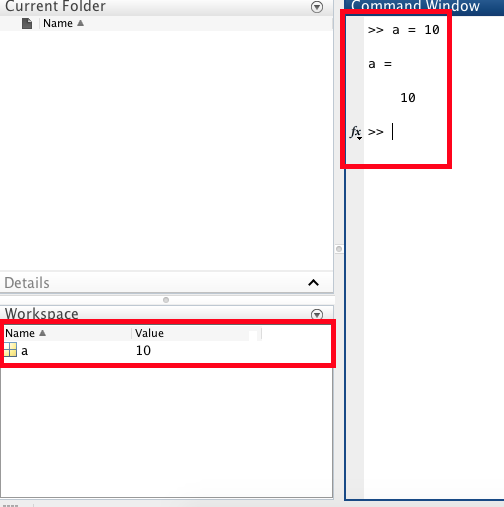
\includegraphics[scale=.5]{hinhtieuluan/pic4}
		\end{center}
		\caption{Tạo biến ở khu vực Command Window và quản lý biến tại khu vực Workspace.}
		\label{refhinh4}
	\end{figure}
\end{center}
\textbf{Ví dụ 2:} Tạo biến c dựa vào biến a có sẵn biết rằng c được tính qua biểu thức $c=a^2+a^3$. Ta tiếp tục nhập lệnh sau vào khu vực Command Window từ ví dụ trước đó:
\begin{lstlisting}
	>> c = a^2 + a^3
	c =
        	1100
\end{lstlisting}
Qua ví dụ 2 ta có thể tạo biến dựa vào giá trị của một biến khác cho trước. Ngoài ra, ta có thể ẩn đi kết quả tính toán của câu lệnh bằng cách thêm dấu ";" vào cuối câu lệnh. Ví dụ sau sẽ giúp ta dễ hình dung:
\begin{lstlisting}
	>> b = 6 + c;
	>> b = 6 + c
	b =
        	1106
\end{lstlisting}

\subsection{Quản lý tập tin, M-file}
\subsubsection{Tạo thư mục lưu trữ}
Trong MATLAB, ta nên tập thói quen dùng các thư mục được sắp xếp gọn gàng để phân loại dữ liệu đang xử lý. Những thao tác cơ bản gồm:
\begin{itemize}
	\item Để tạo thư mục mới, chọn nút "Browse for folder" ở gần khu vực Current Folder. Sau đó ta tạo thư mục mới trong cửa sổ vừa hiện ra, đặt tên cho thư mục (lưu ý rằng tên thư mục không được phép chứa ký tự khoảng trắng).
	\item Chọn thư mục vừa tạo và nhấn nút "Open" để mở.
	\item Lúc này, thư mục hiện hành chính là thư mục bạn vừa mới tạo.
	\item Không chỉ cho phép người dùng tạo thư mục thông qua cửa sổ "Browse for folder", người dùng còn có thể xoá, sửa hay di chuyển thư mục trong cửa sổ đó.
\end{itemize}
\textbf{Nâng cao:} Với những người dùng thường xuyên lưu trữ chương trình hoặc các tập tin m-file ở các thư mục nằm nhiều nơi trên ổ đĩa, người dùng có thể thêm đường dẫn thư mục đó vào cửa sổ \textbf{Set Path (trong phần Enviroment)} để có thể chạy lệnh tính toán mà không cần quan tâm vị trí lưu trữ thư mục chứa các tập tin đó.
\subsubsection{Scripts (Đoạn mã lệnh)}
Scripts (còn được gọi là đoạn mã lệnh, m-hàm hoặc m-file) là một tập tin chứa các câu lệnh chạy trong mội trường MATLAB. Các câu lệnh được lưu trữ trong tập tin này sẽ được thực thi theo trình tự.\\
Scripts được viết trong cửa sổ MATLAB Editor tích hợp sẵn trong MATLAB và được lưu trên ổ đĩa dưới dạng các tập tin có đuôi mở rộng là .m, dung lượng thường chưa đến 100MB. Ngoài ra, ta hoàn toàn có thể dùng một công cụ soạn thảo cơ bản như \textbf{Notepad} mặc định của Windows để tạo ra một tập tin đuôi .m nhưng yêu cầu các câu lệnh trong đó phải đúng và thực thi được trong môi trường MATLAB.\\
Các cách tạo một tập tin MATLAB (đuôi .m):
\begin{itemize}
	\item Từ Command Windows gõ câu lệnh với cú pháp \chuyencode{edit tenfile.m}, trong đó ta thay thế \chuyencode{tenfile.m} bằng tên tập tin muốn tạo. Sau đó chọn OK trong cửa sổ xác nhận tạo tập tin tenfile.m.
	\item Chọn vào biểu tượng \textbf{New Script} trong khu vực \textbf{File} hoặc chọn \menu{File > New > Script} đều được. Sau khi cửa sổ soạn thảo đã mở, ta chọn biểu tượng \textbf{Save} trong khu vực File và tiến hành đặt tên cho tập tin cùng với việc chọn khu vực lưu trữ.
\begin{center}
	\begin{figure}[htp]
		\begin{center}
		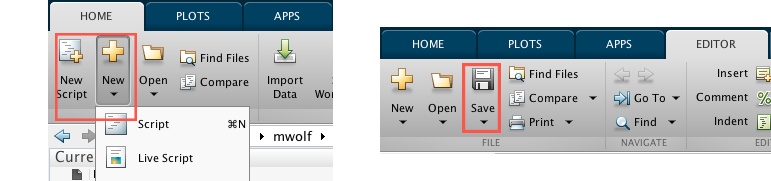
\includegraphics[scale=.5]{hinhtieuluan/pic5}
		\end{center}
		\caption{Khu vực tạo Script mới (hình bên trái) và khu vực lưu Script (hình bên phải).}
		\label{refhinh5}
	\end{figure}
\end{center}
	\item Ngoài hai cách trên, ta còn có thể dùng tổ hợp phím \keys{\ctrl + N} (đối với Windows) hoặc \keys{\cmd + N} (đối với MacOS) để mở cửa số MATLAB Editor và tạo tập tin mới.
\end{itemize}

%Chương 2:
\section{Các thao tác và phép toán với mảng}
%Chương 3:
\section{Vòng lặp điều khiển}
%Chương 4:
\section{Đồ thị trong mặt phẳng và trong không gian}
	%Bìa để sau
	
	%Mục lục
	
	Tiểu luận môn học Phần mềm Toán học

“Một số kiến thức về phần mềm MATLAB”

Chương 1: Cơ bản về MATLAB

1.1  Không gian làm việc

1.2  Biến, câu giải thích, chấm câu

1.3  Các hằng số, các phép toán cơ bản, các hàm toán học.

1.4  Quản lý tập, M-file, M-hàm

(C1 $\rightarrow$ C4)

Chương 2: Các thao tác và phép toán với mảng

(C6 và C7)

Chương 3: Vòng lặp điều khiển (C11)

Chương 4: Đồ thị trong mặt phẳng và trong không gian

(Bổ sung nhiều ví dụ và bài tập)
	%Test cho code
	\begin{lstlisting}
	// Hello.java
	for (i:1);
	import javax.swing.JApplet;
	import java.awt.Graphics;

	public class Hello extends JApplet {
    	public void paintComponent(Graphics g) {
        	g.drawString("Hello, world!", 65, 95);
    	}    
	}
	\end{lstlisting}
	
\end{document}